% Draft for SAFE @ AAAI 2027 (deadline 2026-11-02 AoE), AAAI-27 author kit
% (aaai2027.sty / aaai2027.bst, TemplateVersion 2027.1). The CVPR-template
% version of the same text is main_cvpr.tex. Every number traces to a file
% under docs/ntire/; docs/paper/numbers.md maps each one.
\documentclass[letterpaper]{article} % DO NOT CHANGE THIS
\usepackage[submission]{aaai2027}  % DO NOT CHANGE THIS
\usepackage[hyphens]{url}  % DO NOT CHANGE THIS
\usepackage{graphicx} % DO NOT CHANGE THIS
\urlstyle{rm} % DO NOT CHANGE THIS
\def\UrlFont{\rm}  % DO NOT CHANGE THIS
\usepackage{natbib}  % DO NOT CHANGE THIS AND DO NOT ADD ANY OPTIONS TO IT
\usepackage{caption} % DO NOT CHANGE THIS AND DO NOT ADD ANY OPTIONS TO IT
\frenchspacing  % DO NOT CHANGE THIS
\usepackage{booktabs}
\usepackage{amsmath}
\usepackage{amssymb}

\pdfinfo{
/TemplateVersion (2027.1)
}

\setcounter{secnumdepth}{1} % the template allows 1 or 2

\newcommand{\fov}{\mathrm{FOV}}

\title{Equal Pixels, Unequal Views:\\Field of View Limits Robust AI-Generated Image Detection}
\author{Anonymous Submission}
\affiliations{}

\begin{document}
\maketitle

\begin{abstract}
Detectors built on vision transformers often take a fixed-pixel window at
native resolution, following the field's advice to avoid resizing. The window
fixes pixel count but not field of view: a 200-pixel window sees 39\% of the
short side of a 512-pixel image and 5\% of a 4000-pixel one. On the NTIRE 2026
Robust AI-Generated Image Detection data, the robust ROC AUC of a crop-trained
DINOv2 detector falls as native image size grows. Showing the frozen detector
the whole image raises fused robust AUC on the hard validation split from
0.886 to 0.963, while nine native windows at the same field of view barely
help. The gain appears where the window matches the training field of view,
and retraining the full models under whole-image input adds nothing (0.960),
so it follows
coverage rather than a train-test mismatch. Three controls argue against a
resolution shortcut. A pre-registered repeat with a CLIP ViT-L/14 backbone
gains 14 robust points from whole-image training, 10 of them at test time
alone. On held-out benchmarks the gain holds on AIGIBench SocialRF, is
confounded on CommunityAI, and reverses slightly on Synthbuster near ceiling.
A declared second test read moves robust AUC by +0.062 [+0.040, +0.083] and
clean AUC by $-0.014$ [$-0.024$, $-0.006$], a cost concentrated on large
clean images. B-Free, a public detector built on native-resolution traces,
does not benefit, so we limit the claim to detectors trained with our recipe.
We pre-registered every gate and report two label leaks in public
benchmarks.
\end{abstract}

\section{Introduction}
\label{sec:intro}

Most AI-generated image detectors must turn an image of arbitrary size into a
fixed-size tensor. A long line of forensic work argues that this step should
not resize: ``Most of all, it is important to avoid resizing'' because
interpolation ``may erase the subtle high-frequency traces left by the
generation process'' \cite{corvi2023detection}. The usual answer is a
fixed-pixel window at native resolution, taken once at test time or several
times and averaged \cite{corvi2023detection,li2025safe,guillaro2025bfree,konstantinidou2025texturecrop}.

A fixed-pixel window equalises pixel count. It does not equalise field of
view. We define the field of view of a window of side $s$ on an image with
short side $h$ as $\fov = s/h$. A 200-pixel window covers 39\% of the short
side of a 512-pixel image and 5\% of a 4000-pixel one, so the larger the
image, the less of it the detector sees. FixRes \cite{touvron2019fixres}
describes a related effect in image classification, where a change in
apparent object size between training and test costs accuracy (``networks do
not have built-in scale invariance''). That account, a covariate
shift \cite{shimodaira2000covariate} in the input, predicts that a detector
does best when the test view matches the training view. Ours does not. It
does best when shown the whole image, a view it never trained on, and the
gain appears even where the window already matches the training field of
view. What limits it is coverage: how much of the image it sees.

We found this while building a detector for the NTIRE 2026 Robust
AI-Generated Image Detection challenge \cite{gushchin2026ntire}. Every one of
our 407k training images had a short side between 384 and 512 pixels, so the
200-pixel window we used always covered 39 to 52\% of the short side. On the
organisers' hard validation split it covers as little as 5\%. Our detector's robust AUC fell with
native image size, and three method changes we had pre-registered, aimed at
the degradations, all failed their gates.

\paragraph{Contributions.}
\begin{itemize}
\item A diagnosis. We show that coverage, the share of the image the
  detector sees, limits robust AUC for our ViT detector, and pixel count does
  not. Nine native windows at the same field of view barely help, while one
  whole-image view at the same pixel count gains 7 to 9 AUC points per
  branch. The gain holds where the window already matches the training field
  of view, so it is not a train-test mismatch (Sec.~\ref{sec:diagnosis}). A
  pre-registered repeat on a CLIP backbone shows the same effect, larger
  (Sec.~\ref{sec:training}).
\item A test-time fix with controls. Presenting the whole image to the frozen,
  crop-trained checkpoints recovers the gain with no retraining. Our full
  DINOv2 models gain no more from training under whole-image input; short
  proxy runs gain 4 to 6 points more from it. We test and rule out a
  resolution shortcut three ways, and show the gain on images that received
  no geometric transform (Sec.~\ref{sec:controls}).
\item Pre-registered held-out evidence, including where it fails. Three
  external benchmarks give one clean pass, one confounded pass and one
  failure, and a declared second test read shows a clean-AUC cost on large
  images (Sec.~\ref{sec:heldout}).
\item A pre-registered test on two public detectors. UnivFD is at chance on
  this data, and B-Free fails: whole-image input does not help it and costs
  it clean AUC (Sec.~\ref{sec:public}).
\item Two label leaks in public benchmarks: a file-format and size confound in
  AIGIBench CommunityAI \cite{li2025aigibench}, and a non-monotone size leak in
  the resized RAISE reals commonly paired with
  Synthbuster \cite{bammey2024synthbuster} (Sec.~\ref{sec:leaks}).
\end{itemize}

Whole-image input is not new. The NTIRE 2026 winner resizes the whole image at
inference ``to preserve the global spatial context'', the fifth-placed team
calls its preprocessing ``squish'' \cite{gushchin2026ntire}, and
AI-GenBench \cite{pellegrini2025aigenbench} finds resize ``often preferable''
to multi-crop for CLIP and DINOv2 backbones. None of these works names a
mechanism or tests one. Our contribution is the mechanism and the evidence
for it. We also show where the advice to avoid resizing still holds.

\section{Related work}
\label{sec:related}

\paragraph{Crop, don't resize.} \citet{corvi2023detection} trained
on native patches and fused patch decisions. SAFE \cite{li2025safe} replaces
down-sampling with a crop and reports that the resize ``indeed diminishes the
subtle artifact features''. B-Free \cite{guillaro2025bfree} trains on
504-pixel crops and averages native-resolution crops at test time.
SPAI \cite{karageorgiou2025spai} learns a spectral model so that any
resolution can be scored without resizing. TextureCrop \cite{konstantinidou2025texturecrop}
selects textured native crops and notes that preprocessing loss grows with
native resolution. HiDA-Net \cite{mu2026hidanet} tiles the full image and
reports 84.2\% accuracy from its global view alone against 96.1\% with tiles.
All of these reason about high-frequency traces. SAFE's own ablation is
useful context for us: its CNN scores a centre crop and the full native image
about equally, so a low-level detector does not appear to depend on field of
view.

\paragraph{Resize can win.} AI-GenBench \cite{pellegrini2025aigenbench}
reports resize at least as good as five-crop for fine-tuned DINOv2 ViT-L/14
(94.24 against 93.44 AUROC) and clearly better for CLIP (92.04 against 87.66).
In AIGIBench's test-time comparison \cite{li2025aigibench}, the one CLIP-based
detector does better with resize while all five low-level detectors do better
with crops. \citet{cozzolino2024raising} resize the short side
before a centre crop. WaRPAD \cite{choi2025warpad} rescales the whole image to
a fixed square before tiling it, which holds each tile's field of view
constant, although the paper motivates it differently. GlobalForge \cite{cui2026globalforge}
reports the opposite of our test-time result on clean data: a UnivFD probe
trained with centre crops loses about 8.8 balanced-accuracy points when tested
with resize. We return to this in Sec.~\ref{sec:cost}.

\paragraph{Scale and size as confounds.} \citet{grommelt2024fakeorjpeg}
show that JPEG quality and image size
separate real from fake in GenImage, and note in one sentence that
``detectors employing cropping to achieve a uniform input size are still
subject to bias in terms of object size''. Their concern is a size shortcut
correlated with the label. Ours is the reverse case: size is uninformative in
training and the detector still fails across sizes at test time. \citet{rajan2025aligned}
show that random resized crops inject
resampling signals when real and fake sizes differ, and BIAS-ID \cite{ricker2026biasid}
measures detector score shifts under such transformations. FixRes \cite{touvron2019fixres}
is the closest precedent. Sec.~\ref{sec:diagnosis} shows why its train-test
account does not fit our data.

\section{Setup}
\label{sec:setup}

\paragraph{Data.} We train on 407,223 images: the NTIRE 2026 training shards,
COCO and Open Images reals, and paired real and generated images from several
open and commercial generators. Every training image has a short side of 384 to
512 pixels (median 512). We evaluate on the organisers' labelled splits:
\texttt{ntire\_val} (10,000 images, half distorted), \texttt{ntire\_val\_hard}
(2,500, half distorted) and the public test split \texttt{ntire\_test}
(2,500). Robust AUC is the ROC AUC over distorted images; clean AUC is over
undistorted ones, following the challenge \cite{gushchin2026ntire}.

\paragraph{Models.} Two branches built on DINOv2-L/14 with
registers \cite{oquab2024dinov2,darcet2024registers}, all 24 blocks
fine-tuned, mean-pooled patch tokens, 0.91B parameters in total. Branch A is
one tower at a 512-pixel input, trained for 2 epochs. Branch B concatenates
two towers at 224 pixels, trained for 3 epochs. Each source image yields one
clean view and ten degraded views drawn from a pool of 26 operations in six
families, chained up to five deep, including a neural codec \cite{balle2018hyperprior}
and a downscale applied before the window is taken. The loss is
class-balanced cross-entropy plus a degradation-prediction term (weight 0.3)
and clean-degraded consistency terms on the outputs (KL) and hidden
features (MSE), each at unit weight. The schedule is cosine with 3\% warm-up, with weight
averaging \cite{izmailov2018swa} over the last quarter. On one RTX 4090 the
squish-trained branches took about 19 hours (B) and 29 hours (A).

\paragraph{Input presentation.} The \emph{crop} policy takes a 200-pixel
window at native resolution (the centre window at test time) and resizes it to
the branch's input size. Images with a short side under 200 pixels are taken
whole. The \emph{squish} policy resizes the whole image to the input size,
discarding aspect ratio: area interpolation on the short side down to the input
size when the image is larger, then area interpolation to the square. Both
policies give every image the same number of input pixels. Under squish the
field of view is 1 for every image.

\paragraph{Fusion and selection.} The two branches' logits are z-scored and
combined as $w z_A + (1-w) z_B$. The z-score parameters and the weight $w$ are
fitted on \texttt{ntire\_val} alone, by the mean of robust and clean AUC. For
the squish models the choice between final and averaged weights is made the
same way; for the crop models we kept the choice made earlier on both
validation splits. The fitted weights were $w = 0.50$ for crop and $w = 0.55$
for squish.

\paragraph{Statistics.} All intervals are 95\% percentile intervals from 2,000
paired bootstrap resamples, stratified by label and distortion status, with
the same resample indices for every model being compared.

\paragraph{Protocol.} The test split was read once with the crop fusion
(2026-10-04). We then wrote and committed a pre-registration of the squish
study, with three gates and one declared second test read, before training any
squish model. The gates were: G1, a three-seed proxy comparison; G2, the
fused models on \texttt{ntire\_val\_hard}; and G3, each external benchmark. We
amended the pre-registration four times, each time before the numbers
concerned existed: after inspecting the external data for leaks, to add the
aspect-ratio control (Sec.~\ref{sec:controls}), to score two public detectors
(Sec.~\ref{sec:public}), and to repeat the proxy comparison with a CLIP
backbone (Sec.~\ref{sec:training}). We chose the squish
policy after seeing its effect on \texttt{ntire\_val\_hard}, so that split is
not an unbiased readout of it. The external benchmarks and the test read
carry the held-out evidence. Code, the pre-registration and per-image scores
will be released with the paper.

\section{The diagnosis}
\label{sec:diagnosis}

\begin{table}[t]
\centering
\small
\begin{tabular}{lrrrr}
\toprule
split & n & p5 & p50 & p95 \\
\midrule
train & 407,223 & 0.391 & 0.391 & 0.521 \\
\texttt{ntire\_val} & 10,000 & 0.100 & 0.312 & 0.893 \\
\texttt{ntire\_val\_hard} & 2,500 & 0.112 & 0.298 & 0.784 \\
\bottomrule
\end{tabular}
\caption{Field of view of the 200-pixel window ($200/$short side). Training
is close to a single value. On \texttt{ntire\_val\_hard}, 86.4\% of images
fall outside the training band of 0.391 to 0.521 and 70.8\% fall below it.}
\label{tab:fov}
\end{table}

Table~\ref{tab:fov} shows how much of each image the window covers. In
training it always covers 39 to 52\% of the short side. On
\texttt{ntire\_val\_hard} the median is 30\%, and one image in twenty gets
11\% or less. Under the crop policy, fused robust AUC on
\texttt{ntire\_val\_hard} falls from 0.911 for images with a short side of 80
to 336 pixels to 0.865 for images above 752 pixels. Figure~\ref{fig:size}
shows the same fall in eight equal-count bins.

\begin{figure}[t]
\centering
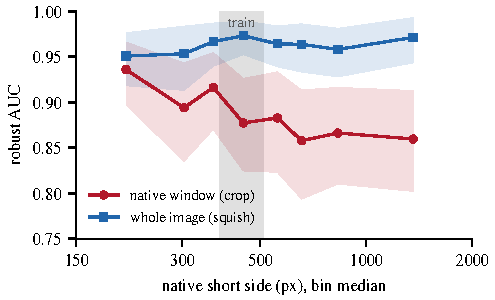
\includegraphics[width=\columnwidth]{fig_size}
\caption{Fused robust AUC on the distorted rows of \texttt{ntire\_val\_hard}
in eight equal-count bins of native short side, with 95\% bootstrap bands.
Red: the crop-trained fusion under its 200-pixel window. Blue: the fusion
trained under squish. Grey: the native short sides of the training images.}
\label{fig:size}
\end{figure}

To separate field of view from pixel coverage, we scored the two frozen
crop-trained branches under four test-time presentations
(Table~\ref{tab:probe}). \emph{grid9} averages nine 200-pixel native windows,
nine times the pixels at the same field of view. \emph{fov3} first downscales
the short side to 600 pixels and then takes the nine windows, which raises the
field of view to $1/3$. \emph{squish} shows the whole image once.

\begin{table}[t]
\centering
\small
\setlength{\tabcolsep}{4pt}
\begin{tabular}{llrrr}
\toprule
branch & presentation & views & robust & clean \\
\midrule
A (512) & centre window & 1 & 0.8561 & 0.9912 \\
        & grid9 & 8.9 & 0.8495 & 0.9978 \\
        & fov3 & 8.9 & 0.8703 & 0.9977 \\
        & squish & 1 & \textbf{0.9482} & 0.9906 \\
\midrule
B (224) & centre window & 1 & 0.8872 & 0.9801 \\
        & grid9 & 8.9 & 0.9049 & 0.9931 \\
        & fov3 & 8.9 & 0.9215 & 0.9942 \\
        & squish & 1 & \textbf{0.9599} & 0.9886 \\
\bottomrule
\end{tabular}
\caption{Frozen crop-trained branches on \texttt{ntire\_val\_hard} under
test-time presentations. More pixels at the same field of view (grid9) help B
by 1.8 points and cost A 0.7. Raising the field of view helps in proportion.}
\label{tab:probe}
\end{table}

More pixels at the same field of view do little: grid9 gains 1.8 robust
points on B and loses 0.7 on A. Gains rise with field of view: fov3 gains 1.4
and 3.4 points, and squish gains 9.2 and 7.3. Squish uses one view and the
same pixel count as the centre window. On B the paired interval for the
squish gain is [+0.057, +0.090]. With z-scores and weight fitted on
\texttt{ntire\_val}, the fused robust AUC rises from 0.886 to 0.963 and the
true positive rate at 1\% false positive rate from 0.516 to 0.752. Clean AUC
moves by $-0.001$ on A and $+0.009$ on B.

\paragraph{Coverage, not mismatch.} A train-test mismatch account, as FixRes
gives for classification, predicts that the crop detector does well wherever
its window matches training. Figure~\ref{fig:size} shows otherwise. In the bin
whose short sides (416 to 496 pixels) lie inside the training range, the
200-pixel window covers the same share of the image as in training, yet the
crop fusion scores 0.877 against 0.973 for squish. Many of these images were
downscaled from larger originals, so their content scale may still differ
from training. Two further results point the same way. Squish shows the
crop-trained branches a field of view of 1, which they never saw in training,
and gains 7 to 9 points. Training the full branches under squish then adds
nothing to that gain (Sec.~\ref{sec:training}). The detector does better the
more of the image it sees, whether or not the view matches training. In
short proxy runs the view match also matters: there, training under squish
adds 4 to 6 points beyond the test-time change, with DINOv2 and with CLIP
(Sec.~\ref{sec:training}).

\section{Is it a resolution shortcut?}
\label{sec:controls}

Squish does not hide native resolution. A small image arrives upsampled and
soft, a large one downsampled and sharp, so a model could read size from the
pixels. Three checks argue that the gain is not size-reading, and two more
show that it does not come from the geometric distortions or from the
stretch.

\paragraph{Size carries no label signal in training.} Native short side scores
an AUC of 0.528 against the label on the training set, where no image exceeds
512 pixels. A shortcut the training data does not reward is unlikely to be
learned.

\paragraph{The gain holds at fixed size.} Within equal-count deciles of native
short side, where the resize factor is nearly constant, squish beats the
centre window in 10 of 10 deciles on branch B. The size-weighted
within-decile robust AUC rises from 0.888 to 0.964, a gain of 7.5 points
against 7.3 pooled.

\paragraph{The gain survives band-limiting.} We band-limit the squished input
to 160 pixels, so native resolution can no longer be read from it. Branch B
keeps all of its gain (+7.2 of +7.3 points). Branch A keeps +5.7 of +9.2. At a
512-pixel input a 160-pixel band removes real detail, so A's shortfall is the
expected cost of the filter.

\paragraph{The gain is not only the geometric distortions.} The challenge's
validation and test splits add random crops, aspect crops, downscaling and
perspective transforms that its training split lacks \cite{gushchin2026ntire}.
These change native size and could carry the effect. Grouping the distorted
rows of \texttt{ntire\_val\_hard} by their transforms
(Table~\ref{tab:groups}), squish gains in every group. On rows that received
only photometric transforms the gain is +9.0 points on A and +8.3 on B, with
intervals clear of zero. Those rows have a median short side of 784 pixels;
large native images are enough to produce the effect.

\begin{table}[t]
\centering
\small
\setlength{\tabcolsep}{3pt}
\begin{tabular}{lrrcc}
\toprule
distortions & n & short p50 & A gain & B gain \\
\midrule
photometric only & 241 & 784 & +0.090 & +0.083 \\
downscale, no crop & 740 & 432 & +0.095 & +0.065 \\
crop or aspect crop & 191 & 320 & +0.059 & +0.063 \\
perspective & 78 & 536 & +0.146 & +0.140 \\
\bottomrule
\end{tabular}
\caption{Squish gain in robust AUC over the centre window, within groups of
distorted \texttt{ntire\_val\_hard} rows, frozen crop-trained branches. All
eight 95\% intervals exclude zero.}
\label{tab:groups}
\end{table}

\paragraph{Aspect ratio.} Squish stretches non-square images, which
\citet{grommelt2024fakeorjpeg} warn introduces frequency artefacts
along one axis. To attribute the gain to field of view
rather than to the stretch, we registered two aspect-preserving presentations
before scoring them: \emph{short-centre} (short side to the input size, then
the centre square) and \emph{letterbox} (long side to the input size, padded
to a square). We predicted that each would recover at least 75\% of squish's
gain on both branches. Both did (Table~\ref{tab:aspect}): short-centre kept
93\% of the gain on A and 97\% on B, letterbox 100\% and 94\%. Against squish,
short-centre is 0.7 points lower in robust AUC on A, with an interval that
excludes zero, and indistinguishable on B. Letterbox matches squish in robust
AUC but loses 0.4 points of clean AUC on both branches. The stretch is
therefore not what drives the gain; showing the whole short side is.

\begin{table}[t]
\centering
\small
\setlength{\tabcolsep}{3pt}
\begin{tabular}{lcccc}
\toprule
 & \multicolumn{2}{c}{robust gain over centre} & \multicolumn{2}{c}{clean vs.\ squish} \\
\cmidrule(lr){2-3}\cmidrule(lr){4-5}
presentation & A & B & A & B \\
\midrule
squish & +0.092 & +0.073 & -- & -- \\
short-centre & +0.085 & +0.070 & 0.000 & 0.000 \\
letterbox & +0.092 & +0.069 & $-0.004$* & $-0.004$* \\
\bottomrule
\end{tabular}
\caption{Differences in AUC for the aspect-preserving presentations, with the
frozen crop-trained branches on \texttt{ntire\_val\_hard} and a paired
bootstrap of 2000 resamples. Every robust gain
has a 95\% interval that excludes zero. * marks a clean difference whose
interval excludes zero.}
\label{tab:aspect}
\end{table}

\section{Does training on whole images help?}
\label{sec:training}

\paragraph{Proxy (G1).} We trained matched pairs of single-tower models for
one epoch on a quarter of the training set, differing only in presentation,
at three seeds. On \texttt{ntire\_val\_hard}, squish beat crop by +0.083
[+0.062, +0.105], +0.093 [+0.072, +0.115] and +0.078 [+0.057, +0.102] robust
AUC, with clean AUC within noise (+0.008 to +0.012, every interval spanning
zero). On \texttt{ntire\_val} the robust gain was +0.035 to +0.037. All three
pre-registered conditions held, so we trained the full branches.

\paragraph{Full branches.} Table~\ref{tab:branches} compares, per branch, the
crop-trained model under its own presentation, the same frozen model under
squish, and the model trained under squish. Training under squish matches the
test-time change on robust AUC (A: 0.943 against 0.948; B: 0.959 against
0.960) and adds a little clean AUC. The fused squish-trained models reach
0.960 robust and 0.995 clean on \texttt{ntire\_val\_hard}, against 0.886 and
0.990 for the crop fusion: +0.074 [+0.058, +0.091] robust (G2). The size
gradient is gone: across the four size buckets the squish fusion scores 0.951,
0.971, 0.965 and 0.967, and across the eight bins of Figure~\ref{fig:size} it
stays between 0.951 and 0.973.

\begin{table}[t]
\centering
\small
\setlength{\tabcolsep}{4pt}
\begin{tabular}{llcc}
\toprule
branch & model & robust & clean \\
\midrule
A & crop-trained & 0.8561 & 0.9913 \\
  & crop-trained, squish at test & 0.9482 & 0.9906 \\
  & squish-trained & 0.9425 & 0.9934 \\
\midrule
B & crop-trained & 0.8873 & 0.9801 \\
  & crop-trained, squish at test & 0.9599 & 0.9886 \\
  & squish-trained & 0.9589 & 0.9898 \\
\bottomrule
\end{tabular}
\caption{Per branch on \texttt{ntire\_val\_hard}. Training under squish adds
nothing to robust AUC beyond presenting the whole image to the crop-trained
model. Paired gains over crop-trained: A +0.092 and +0.086, B +0.073 and
+0.072, all intervals clear of zero. The crop-trained rows were rescored for
this table and differ from Table~\ref{tab:probe} by at most 0.0001.}
\label{tab:branches}
\end{table}

\paragraph{A second backbone.} Our fourth amendment repeated G1 with a CLIP
ViT-L/14 tower \cite{radford2021clip} in place of DINOv2, every other setting
unchanged (including ImageNet input normalisation). It added two tests: the
crop-trained checkpoints shown the whole image at test time, and a mechanism
check requiring the gain above 752 pixels of short side to exceed the gain
below 336. Table~\ref{tab:clip} gives the means over three seeds, and every
registered test passed. Training under squish beat crop by +0.144, +0.150 and
+0.139 robust AUC, every interval clear of zero, with clean AUC unchanged
(mean $-0.001$, every interval spanning zero). At test time alone the gain
was +0.096, +0.111 and +0.094, again clear of zero. Both gains grow with
size: +0.206 above 752 pixels against +0.091 below 336 for training, and
+0.168 against +0.057 at test time. CLIP's crop-trained proxies are weaker
than DINOv2's (0.748 robust against 0.799) and gain more.

The CLIP results led us to run the same test-time comparison on the DINOv2
proxies, which we had not registered. Shown the whole image, the DINOv2
crop-trained proxies gain +0.026 to +0.038 robust AUC, every interval clear
of zero, and the gain again grows with size (+0.075 above 752 pixels, +0.023
below 336). At proxy scale, training under squish adds to the test-time
change for both backbones: squish-trained proxies beat the crop-trained ones
shown the whole image by +0.048 to +0.057 robust and +0.022 to +0.032 clean
with DINOv2, and by +0.038 to +0.048 and +0.025 to +0.040 with CLIP, every
interval clear of zero. Test-time squish costs the crop-trained proxies 1 to
4 clean points, which training recovers. The full DINOv2 branches show no
such gap (Table~\ref{tab:branches}). They differ from the proxies in training
length, number of views per image and loss terms, and we cannot say which
of these closes the gap.

\begin{table}[t]
\centering
\small
\setlength{\tabcolsep}{4pt}
\begin{tabular}{llcc}
\toprule
backbone & model & robust & clean \\
\midrule
DINOv2 & crop-trained & 0.7994 & 0.9255 \\
       & crop-trained, squish at test & 0.8310 & 0.9087 \\
       & squish-trained & 0.8841 & 0.9357 \\
\midrule
CLIP & crop-trained & 0.7482 & 0.9655 \\
     & crop-trained, squish at test & 0.8485 & 0.9324 \\
     & squish-trained & 0.8924 & 0.9645 \\
\bottomrule
\end{tabular}
\caption{Proxy models (one tower, one epoch on a quarter of the training set)
on \texttt{ntire\_val\_hard}, mean of three seeds. The DINOv2 test-time row
was not registered.}
\label{tab:clip}
\end{table}


\section{Held-out evidence}
\label{sec:heldout}

\subsection{External benchmarks (G3)}

We scored three external benchmarks that no model was trained or selected on,
after removing any image whose content digest matched an NTIRE image:
AIGIBench SocialRF and CommunityAI \cite{li2025aigibench}, and Synthbuster
with RAISE-1k reals \cite{bammey2024synthbuster,dangnguyen2015raise}. All three
are clean, so we report pooled AUC on the files as distributed (the gate), on
every file re-encoded as JPEG at quality 95, and on every file passed through
one seeded chain from our degradation pool. That last reading is our own
synthesis, not the organisers', and it is not a gate.

\begin{table*}[t]
\centering
\small
\begin{tabular}{lccc}
\toprule
 & SocialRF & CommunityAI & Synthbuster \\
\midrule
n (real/fake) & 2994/3000 & 6000/6000 & 994/8996 \\
short side p50 & 1366 & 500 & 833 \\
size-label AUC & 0.694 & 0.916 & 0.519 \\
format-label AUC & 0.500 & 1.000 & 0.555 \\
\midrule
crop fusion & 0.9633 & 0.9809 & 0.9995 \\
squish fusion & 0.9776 & 0.9920 & 0.9984 \\
difference (G3) & +0.014 & +0.011 & $-0.001$ \\
\quad 95\% CI & [+0.010, +0.018] & [+0.009, +0.013] & [$-0.002$, $-0.001$] \\
\midrule
size-matched, JPEG 95 & +0.016 & +0.005 & n/a \\
\quad 95\% CI & [+0.009, +0.024] & [$-0.002$, +0.012] & \\
degraded (ours) & +0.085 & +0.070 & +0.024 \\
\bottomrule
\end{tabular}
\caption{External benchmarks, fused AUC. Size-matched is the size-weighted AUC
within deciles of native short side. It cannot be computed on Synthbuster
because no decile holds both classes (Sec.~\ref{sec:leaks}).}
\label{tab:external}
\end{table*}

Table~\ref{tab:external} gives the results. On SocialRF, squish wins on the
files as distributed, after JPEG re-encoding, and within size deciles. On
CommunityAI the pooled gain passes the gate, but every real image is a JPEG
and every fake a PNG, and native size alone separates the classes with AUC
0.916. Our first amendment required the size-matched gain on the re-encoded
files to clear zero before CommunityAI could count as support. It does not
([$-0.002$, +0.012]), so we report CommunityAI as confounded. On Synthbuster
squish loses by 0.001, with both fusions near ceiling. Under our degradation
chains squish wins on all three sets, by 2.4 to 8.5 points.

\subsection{The second test read}

Table~\ref{tab:test} gives both reads of the public test split. Read 1 used the
crop fusion as frozen on 2026-09-23 and read on 2026-10-04. Read 2 used the squish fusion as frozen
before any squish model was scored on test, and our pre-registration allows no
third read. Robust AUC rose by +0.062 [+0.040, +0.083] and clean AUC fell by
0.014 [0.006, 0.024]. On robust AUC the squish fusion would sit between the
sixth- and seventh-placed challenge entries on the open test, where the crop
fusion was below all nine; we were not a challenge entry and make no ranking
claim. The leading entries use far more compute, such as committees of DINOv3
models at 512 pixels on 32 A100 GPUs \cite{gushchin2026ntire}.

\begin{table}[t]
\centering
\small
\begin{tabular}{lcccc}
\toprule
read & robust & clean & AUC & TPR@1\% \\
\midrule
1, crop & 0.7931 & 0.9856 & 0.9108 & 0.289 \\
2, squish & 0.8547 & 0.9715 & 0.9211 & 0.300 \\
\bottomrule
\end{tabular}
\caption{The two reads of \texttt{ntire\_test} (2,500 images). Read 1's fusion
weight was fitted on both validation splits ($w = 0.45$); read 2's on
\texttt{ntire\_val} alone.}
\label{tab:test}
\end{table}

\section{Where whole-image input costs}
\label{sec:cost}

The clean loss on the test split has one source. Split by native size, clean
AUC of branch A on test images with a short side above 1100 pixels falls from
0.974 under crop to 0.880 under squish (366 images). Below 1100 pixels, and on
branch B at every size, the change is under 1.3 points. The real images are not
the cause: under crop their mean score drifts toward ``fake'' as size grows,
and under squish it is flat. The fake images are: their mean score under
squish falls with size.

The validation splits do not show this cost. On their clean images above
1100 pixels, branch A trained under squish scores 1.000 against 0.989 for
crop on \texttt{ntire\_val} (871 images) and 0.978 against 0.981 on
\texttt{ntire\_val\_hard} (295 images). Something about the test split's large
generated images differs, and the split carries no generator labels, so we
cannot say what. Our hypothesis is the trade-off the forensic literature
predicts: a clean, large generated image keeps fine traces at native
resolution, and reducing it to 512 pixels discards them. This would also
reconcile our result with GlobalForge \cite{cui2026globalforge} and
TextureCrop's CLIP results \cite{konstantinidou2025texturecrop}, both measured
on clean data. Once blur, compression or downscaling has damaged the traces,
the detector has to judge content, and content needs context. We have not
tested this hypothesis directly.

\section{Public detectors}
\label{sec:public}

To test whether the effect reaches beyond our detector, we registered a third
amendment before scoring two public checkpoints. UnivFD \cite{ojha2023univfd}
is a linear probe on CLIP ViT-L/14 features, trained on 224-pixel crops of
256-pixel images. B-Free \cite{guillaro2025bfree} is a DINOv2-B with
registers that averages five 504-pixel token windows taken at native
resolution. We scored each three ways: its authors' test pipeline (native),
its own training field of view (short side to its training size, then its
crop), and squish at its input size. The primary test was squish minus native
in robust AUC on \texttt{ntire\_val\_hard}, with an interval that excludes
zero. If no presentation reached 0.60 robust AUC, we would report the numbers
and not interpret them.

UnivFD is at chance on NTIRE data under every presentation (robust AUC 0.49 to
0.51 on the hard split). That is below the floor, so it says nothing either
way.

B-Free fails the primary test (Table~\ref{tab:public}). Squish changes its
robust AUC on the hard split by $-0.018$ [$-0.041$, +0.004], and the change
falls with image size instead of rising: $-0.098$ for short sides above 752
pixels, +0.014 below 336. Both resized presentations lower B-Free's clean AUC
on every split, by 1.2 to 18.8 points, which is what the advice to avoid
resizing predicts for a detector built on native-resolution traces (the
range covers the splits in Table~\ref{tab:public}). Two
results go the other way: its training field of view gains 1.9 robust points
[+0.9, +2.9] on \texttt{ntire\_val}, and squish gains 6.3 points [+5.1, +7.5]
on SocialRF under our degradation chains. As registered, we narrow the claim.
Coverage limits the crop-trained detectors we fine-tuned from DINOv2 and from
CLIP; we have no evidence that it limits a detector designed around
native-resolution traces.

\begin{table}[t]
\centering
\small
\setlength{\tabcolsep}{4pt}
\begin{tabular}{lccc}
\toprule
split & native & train FOV & squish \\
\midrule
hard-val, robust & 0.636 & 0.631 & 0.618 \\
hard-val, clean & 0.909 & 0.753 & 0.722 \\
\texttt{ntire\_val}, robust & 0.735 & 0.754 & 0.744 \\
\texttt{ntire\_val}, clean & 0.920 & 0.848 & 0.825 \\
\midrule
SocialRF & 0.922 & 0.889 & 0.871 \\
\quad degraded (ours) & 0.757 & 0.829 & 0.820 \\
CommunityAI & 0.891 & 0.742 & 0.703 \\
\quad degraded (ours) & 0.683 & 0.568 & 0.539 \\
Synthbuster & 0.998 & 0.987 & 0.976 \\
\quad degraded (ours) & 0.896 & 0.893 & 0.892 \\
\bottomrule
\end{tabular}
\caption{B-Free AUC under three presentations. Native is the authors' own
five-window test pipeline. Hard-val is \texttt{ntire\_val\_hard}.}
\label{tab:public}
\end{table}

\section{Two label leaks}
\label{sec:leaks}

\paragraph{AIGIBench CommunityAI.} All 6,000 real images are JPEG files and all
6,000 fake images are PNG files, so container format separates the classes
perfectly, and native short side separates them with AUC 0.916. We found no
mention of this in the paper or its public issue trackers. Results on this
subset should be reported after format equalisation and within size strata.

\paragraph{Synthbuster with resized RAISE reals.} Synthbuster ships only
generated images \cite{bammey2024synthbuster}. A widely used copy of its RAISE
reals was resized so that each image's area is about $1024^2$
pixels \cite{guillaro2025bfree}; we used this copy. All 994 reals then have a
short side of 833 to 835 pixels, while the fakes range from 256 to 2048. The
monotone size-label AUC is 0.519 because the reals sit in the middle of the
fakes' range, but the rule ``short side within 833 to 835'' separates the
classes almost perfectly. A monotone leak check misses this. In the same
benchmark, Adobe Firefly images saved with a \texttt{.png} extension are JPEG
internally \cite{ricker2026biasid}; 997 of our fakes are JPEG.

\section{What did not help}

Before finding the coverage effect we pre-registered three changes aimed
at the degradations, each with a written gate. Distilling degraded features
toward clean ones lost about one robust point on the proxy, and under a
control that gave both views the same window it still gained nothing
($-0.2$ points against a gate of $+1$).
Conditioning the classifier on a predicted degradation embedding through FiLM
tied the baseline (0.803 against 0.804). Weighting the fusion by predicted
degradation severity could not clear its gate of $+0.5$ points even with an
oracle (+0.4 points pooled). These are single-proxy results, but together with the probe they
suggest the representation was not the bottleneck.

\section{Limitations}

Our full models use one backbone (DINOv2-L with registers) at two input
sizes. The CLIP repeat is at proxy scale only, and both backbones went
through our own fine-tuning recipe. The
low-level detectors that motivate the advice to avoid resizing may not share
the effect, and SAFE's results suggest they do not \cite{li2025safe}. The
policy was chosen on \texttt{ntire\_val\_hard}, so its numbers there are
optimistic; the external sets and the test read are the unbiased evidence,
and they are mixed. We have not shown why coverage matters on degraded
images; our hypothesis, that degradations damage local traces and leave the
detector to judge content spread across the image, is untested. The clean
cost on large images is real and is not addressed here. Combining a whole-image view with native windows, as
HiDA-Net and GLASS do \cite{mu2026hidanet,han2026glass}, is the obvious next
step, but it would need its own held-out test. Of the two public detectors we
tested, one is at chance on this data and the other does not benefit
(Sec.~\ref{sec:public}), so we have not shown the effect outside our own
training recipe.

\section{Conclusion}

A fixed-pixel window at native resolution fixes pixel count and leaves field
of view free: the larger the image, the smaller the share the detector sees.
For our DINOv2 detector on degraded images, that share limited robust AUC,
not the representation and not a mismatch with the training view. Showing
the whole image recovered 7 to 9 points per branch with no retraining, and
training the full models on whole images added nothing more. In short proxy
runs, CLIP and DINOv2 backbones both gained at test time (10 and 3 points)
and more from training (4 and 5). On the
test split's clean, large images the same change cost clean AUC, possibly the
case the advice to avoid resizing was written for. B-Free, which follows that
advice, lost clean AUC under every resized presentation and gained no robust
AUC on the hard split. Detection papers should report the field of
view their preprocessing implies, alongside resolution and crop policy.

\bibliography{refs}

\end{document}
